The system architecture developed for object manipulation is focused on grasping. In the implementation, its input is a specific target entity in \acrshort{ed}, selected by a Python executive and the output is the grasp motion joint trajectory.
Figure \ref{fig:grasping_pipeline} shows the grasping pipeline.
\begin{figure}[H]
    \centering
    %\vspace{-0.3cm}
	\includegraphics[width = 1\linewidth]{Figures/grasping_pipeline}
    %\vspace{-1em}
	\caption{Custom grasping pipeline base on \acrshort{ed}, MoveIt and a separate grasp point determination and approach vector node.}
	\label{fig:grasping_pipeline}
    %\vspace{-0.5cm}
\end{figure}
\noindent MoveIt! is used to produce joint trajectories over time, given the current configuration, robot model, \acrshort{ed} world model (for collision avoidance) and the final configuration.
%\acrshort{ed} provides collision meshes to MoveIt! so it can plan paths that avoid obstacles.
%Finally, the trajectories are sent to the reference interpolator which sends the trajectories either to the controllers or the simulated robot.
%The grasping pipeline is extended with an empty spot designator and grasping pose determination. The empty spot designator searches in an area, like `on-top-of'of the dinner table, for an empty spot to place an object by using the occupied area by other objects in this area.
The grasp pose determination uses the information about the position and shape of the object in \acrshort{ed} to determine the best grasping pose.
The grasping pose is a vector relative to the robot.
%An example of the determined grasping pose is shown in Figure \ref{fig:grasping_pose_determination}.
Placing an object is approached in a similar manner to grasping, except for that when placing an object, \acrshort{ed} is queried to find an empty placement pose.

%
%\begin{figure}[H]
%   \centering
%   %\vspace{-0.3cm}
%   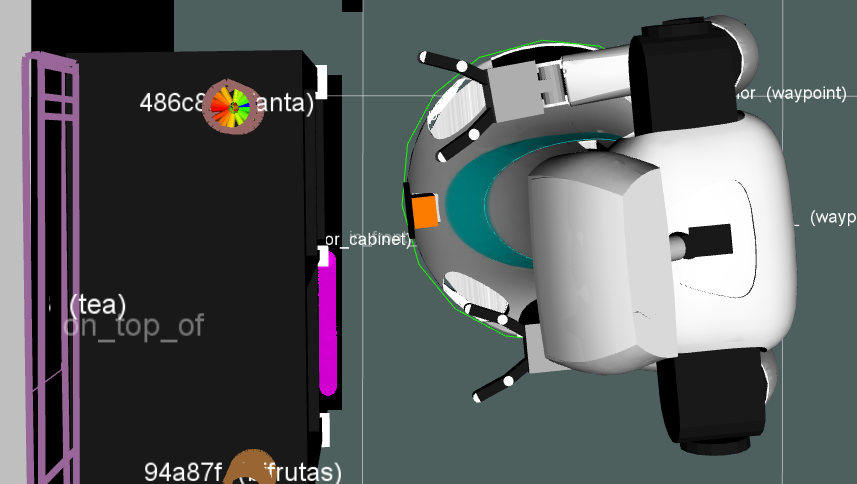
\includegraphics[width = 0.8\linewidth]{Figures/grasp_point_determination}
%    %\vspace{-1em}
%	\caption{Grasping pose determination result for a cylindric object with %TU/e built robot AMIGO. It is unpreferred to grasp the object from behind.}
%	\label{fig:grasping_pose_determination}
%    %\vspace{-0.5cm}
%\end{figure}
